% docs/slides/preamble.tex -- 五份 deck 共享
\documentclass[aspectratio=169,11pt]{beamer}

% ==== 中文与字体 ====
\usepackage[UTF8,fontset=none]{ctex}
\usepackage{fontspec}

\IfFontExistsTF{PingFang SC}{%
  \setCJKmainfont{PingFang SC}[BoldFont=PingFang SC,ItalicFont=PingFang SC,AutoFakeSlant=0.15]
  \setCJKsansfont{PingFang SC}[ItalicFont=PingFang SC,AutoFakeSlant=0.15]
  \setCJKmonofont{PingFang SC}
}{%
  \IfFontExistsTF{Source Han Sans SC}{%
    \setCJKmainfont{Source Han Sans SC}
    \setCJKsansfont{Source Han Sans SC}
  }{%
    \IfFontExistsTF{Noto Sans CJK SC}{%
      \setCJKmainfont{Noto Sans CJK SC}
      \setCJKsansfont{Noto Sans CJK SC}
    }{%
      \setCJKmainfont{Heiti SC}
      \setCJKsansfont{Heiti SC}
    }
  }
}

\IfFontExistsTF{Helvetica Neue}{\setmainfont{Helvetica Neue}}{%
  \IfFontExistsTF{Inter}{\setmainfont{Inter}}{}}
\IfFontExistsTF{JetBrains Mono}{\setmonofont{JetBrains Mono}[Scale=0.85]}%
  {\setmonofont{Menlo}[Scale=0.85]}

% ==== 颜色 ====
\usepackage{xcolor}
\definecolor{cMain}{HTML}{1F4E79}
\definecolor{cAccent}{HTML}{E07A1F}
\definecolor{cGray}{HTML}{595959}
\definecolor{cMute}{HTML}{F4F4F4}
\definecolor{cOK}{HTML}{2E7D32}
\definecolor{cBad}{HTML}{B23A3A}
\definecolor{cWarn}{HTML}{C8A300}

% ==== 主题 ====
\usepackage{tcolorbox}
\usetheme{metropolis}
\metroset{progressbar=frametitle,numbering=fraction,block=fill}
\setbeamercolor{frametitle}{bg=cMain,fg=white}
\setbeamercolor{progress bar}{fg=cAccent,bg=cMute}
\setbeamercolor{alerted text}{fg=cAccent}
\setbeamercolor{title}{fg=cMain}

% metropolis 默认尝试 Fira Sans，未安装时 fallback 到 Latin Modern Sans。
% 这里在主题加载后显式覆盖，强制使用 macOS 上一定存在的 Helvetica Neue，
% 跟中文 PingFang 风格一致；找不到则按顺序尝试 Inter / Arial。
\IfFontExistsTF{Helvetica Neue}{%
  \setsansfont{Helvetica Neue}%
}{%
  \IfFontExistsTF{Inter}{\setsansfont{Inter}}{%
    \IfFontExistsTF{Arial}{\setsansfont{Arial}}{}}%
}

% ==== TikZ ====
\usepackage{tikz}
\usetikzlibrary{positioning,arrows.meta,fit,shapes.geometric,calc,%
  decorations.pathmorphing,backgrounds}

\tikzset{
  node-box/.style={draw=cMain,thick,rounded corners=2pt,
    minimum height=8mm,minimum width=18mm,align=center,font=\small},
  node-state/.style={draw=cMain,thick,circle,minimum size=14mm,
    align=center,font=\small},
  node-ok/.style={draw=cOK,thick,fill=cOK!10},
  node-warn/.style={draw=cWarn,thick,fill=cWarn!15},
  node-bad/.style={draw=cBad,thick,fill=cBad!10},
  % 色盲友好的状态机三态：蓝 (正常/Closed) / 橙 (告警/Open) / 灰 (中间/HalfOpen)
  % 避免 red-green 二元区分，改用 hue + lightness 双通道。
  node-state-normal/.style={draw=cMain,thick,fill=cMain!12},
  node-state-alert/.style={draw=cAccent,thick,fill=cAccent!18},
  node-state-transition/.style={draw=cGray,thick,fill=cGray!18},
  arrow/.style={-{Stealth[length=2mm]},thick,draw=cMain},
  arrow-async/.style={-{Stealth[length=2mm]},thick,dashed,draw=cGray},
  arrow-bad/.style={-{Stealth[length=2mm]},thick,draw=cBad},
  arrow-alert/.style={-{Stealth[length=2mm]},thick,draw=cAccent},
  lifeline/.style={dashed,thick,draw=cGray},
}

% ==== 代码 ====
\usepackage{listings}
\lstdefinelanguage{Go}{
  morekeywords={break,case,chan,const,continue,default,defer,else,
    fallthrough,for,func,go,goto,if,import,interface,map,package,range,
    return,select,struct,switch,type,var,nil,true,false,iota},
  morekeywords=[2]{string,int,int64,uint,uint64,bool,byte,error,context},
  sensitive=true,
  morecomment=[l]//,morecomment=[s]{/*}{*/},
  morestring=[b]",morestring=[b]`,
}
\lstdefinelanguage{LuaRedis}{
  morekeywords={and,break,do,else,elseif,end,false,for,function,if,in,
    local,nil,not,or,repeat,return,then,true,until,while},
  morekeywords=[2]{redis,call,KEYS,ARGV,tonumber,HGET,HSET,GET,SET,
    DECR,DECRBY,INCR,INCRBY,EXPIRE,PEXPIRE,ZADD,ZCARD,ZREMRANGEBYSCORE,
    EVAL,EVALSHA},
  sensitive=true,
  morecomment=[l]{--},
  morestring=[b]",morestring=[b]',
}

\lstdefinestyle{base}{
  basicstyle=\ttfamily\scriptsize,
  numbers=left,numberstyle=\tiny\color{cGray},
  keywordstyle=\color{cMain}\bfseries,
  keywordstyle=[2]\color{cAccent},
  stringstyle=\color{cOK},
  commentstyle=\color{cGray}\itshape,
  backgroundcolor=\color{cMute},
  frame=single,framerule=0pt,
  showstringspaces=false,
  breaklines=true,
  tabsize=2,
  columns=fullflexible,
}
\lstset{style=base}

% ==== 三线表与附录页码 ====
\usepackage{booktabs}
\usepackage{appendixnumberbeamer}

% ==== 页脚来源标注 ====
\newcommand{\srcnote}[1]{{\color{cGray}\scriptsize\itshape #1}}

% 关键论点框
\newcommand{\keypoint}[1]{%
  \begin{tcolorbox}[colback=cMute,colframe=cMain,boxrule=0.5pt,arc=2pt]%
  #1\end{tcolorbox}}


\title{Web3 支付：业务通道、托管增信、对账兜底}
\subtitle{gomall 把"第三方支付吃不下的订单"接回来：跨境 / 加密原生 / 大额托管}
\author{gomall · 业务侧 deck}
\date{}

\begin{document}

\maketitle

\begin{frame}{今日大纲}
\tableofcontents
\end{frame}

% ============================================================
\section{业务定位：Web3 不是新潮，是"补一块法币吃不下的市场"}
% ============================================================

\begin{frame}{先讲清楚 gomall 为什么开 Web3 通道}
\textbf{不是为了潮，不是为了讲技术，是为了三类订单}：
\begin{itemize}
  \item \textbf{加密原生用户}：钱包里只有 ETH / USDT，没绑卡也没法绑卡（行业数据：DeFi 月活 5--7M 钱包），传统通道直接把他们挡在门外。
  \item \textbf{跨境订单}：买家在东南亚 / 拉美 / 非洲，传统跨境 Visa / SWIFT 收 1--3\% 手续费 + T+1 到账，争议解决靠银行流程长达 30--90 天。
  \item \textbf{大额托管交易}：单笔 \$1{,}000+ 跨境订单，买卖双方互不信任、传统支付牌照机构不愿担保，需要"中介信任"换"代码不变式"。
\end{itemize}
\vspace{1mm}
\small Web3 通道与法币 \texttt{/paydown} \textbf{并存}，不是替换。开新通道 = 拓客，不是减客。
\srcnote{routes/router.go:122--136 paydown（法币）与 paydown/crypto（web3）平行挂载}
\srcnote{README.md:69--80 业务边界："不真上链"是显式声明的范围}
\end{frame}

\begin{frame}{5 角色视角：Web3 通道对每个角色意味着什么}
\begin{tabular}{@{}lll@{}}
\toprule
角色 & 在 Web3 通道里关心什么 & 主要痛点 \\
\midrule
C 端用户 & 钱安全吗 / 链上钱付了为什么还没到 & "pending 半小时是不是丢了" \\
商家   & 我什么时候确认到账 / 谁出 gas    & T+0 vs 法币 T+1，但 gas 自付有疑虑 \\
运营   & 开通道能多接多少订单             & 拓客转化率 / 客单价 \\
客服   & 用户骂"网络回滚我钱呢"咋办      & 需要 reorg / pending 的话术 \\
SRE    & 链是不可靠通道，掉块怎么办       & listener catch-up / 退避 / 多源 \\
\bottomrule
\end{tabular}
\vspace{2mm}
\small \textbf{业务承诺要分角色给}：用户要的是"钱在哪我能查"，商家要的是"什么时候 release"，
客服要的是"按业务码读话术不掉链子"，SRE 要的是"链断 30 分钟主流程不挂"。
\srcnote{README.md:21--29 5 角色业务全景表}
\end{frame}

\begin{frame}{业务价值定量：开一条 Web3 通道相当于开三个用户群}
\begin{tabular}{@{}lll@{}}
\toprule
新用户群 & 行业体量参考 & gomall 接入收益 \\
\midrule
DeFi 原生  & 月活 5--7M 钱包 & 钱包内资产可直接付款，零卡组织摩擦 \\
跨境（拉美 / 东南亚 / 非洲） & 跨境电商 GMV 年增 13\% & 1--3\% 手续费 $\to$ gas 固定，T+1 $\to$ 1--2 分钟 \\
大额 B2B 托管 & 单笔 \$1k--\$50k & 中介信任 $\to$ 合约不变式，争议有链上证据 \\
\bottomrule
\end{tabular}
\vspace{2mm}
\small 数字不用记牢，记住一句：\textbf{Web3 不是替代第三方支付，是补齐法币吃不下的订单形态}。
法币通道仍跑 \texttt{/paydown}（deck 05），Web3 通道跑 \texttt{/paydown/crypto}，两条线并行。\\
\textbf{业务边界对外坦白}：MVP 阶段默认不接 RPC（\texttt{WEB3\_RPC\_URL} 不设 listener 不启动），合约 + binding 已就绪。
\srcnote{routes/router.go:122--136 法币 + Web3 两条支付通道并行}
\srcnote{README.md:75--80 不真上链是显式业务边界}
\end{frame}

\begin{frame}{跨境用户旅程：东南亚买家在 gomall 下单的真实链路}
\textbf{角色}：印尼买家 Andi，钱包里有 USDT，要买一台 \$280 的中国卖家相机。
\begin{itemize}
  \item \textbf{法币通道（不可行）}：当地银行卡跨境刷卡费 2.5\% + 汇率损耗 1\%；到账 T+1；纠纷 30--90 天。
  \item \textbf{Web3 通道}：钱包签名 $\to$ \texttt{fundWithOrderID} 把 USDT 锁进 escrow $\to$ 1--2 分钟链上确认 $\to$ 商家发货 $\to$ Andi 收到货确认 \texttt{release} $\to$ 卖家拿到 USDT。
  \item \textbf{时间窗对比}：法币通道 1 周资金锁定 + 1\% 手续费；Web3 通道 1--2 分钟到账 + gas \$0.05--\$0.30（L2）。
  \item \textbf{争议处理}：传统 chargeback 走 Visa 流程 30--60 天，结果靠平台 / 银行裁；Web3 escrow 走 \texttt{dispute} 状态 $\to$ arbiter 在链上裁决，证据是不可篡改的链上事件。
\end{itemize}
\vspace{1mm}
\small 业务收益：\textbf{平台多接一类跨境订单}（DeFi 钱包用户 + 跨境无卡用户），手续费收入从买家结算端转到链上 gas（用户自付），平台净抽成空间反而提升。
\srcnote{contracts/Escrow.sol:68--82 fund；:85--107 release/refund/dispute 状态出口}
\srcnote{routes/router.go:122--136 法币 + Web3 通道并行}
\end{frame}

\begin{frame}{运营视角：开 Web3 通道的转化数据怎么追}
\textbf{运营要回答两个业务问题}：
\begin{itemize}
  \item \textbf{Q1：开 Web3 通道带来多少新用户？}
  \begin{itemize}
    \item 埋点：注册流里"绑定钱包"按钮的点击率 / 完成率；
    \item 看板：每日新增钱包绑定用户 / Web3 支付 GMV / Web3 通道 ARPU；
    \item 决策：如果 Web3 通道 GMV $<$ 平台总 GMV 的 1\%，是否关闭通道节约 RPC 成本？
  \end{itemize}
  \item \textbf{Q2：Web3 通道的转化漏斗在哪卡？}
  \begin{itemize}
    \item 漏斗：进入支付页 $\to$ 选 Web3 $\to$ 钱包签名成功 $\to$ 链上 fund $\to$ 6 块确认；
    \item gomall 当前实现：每步都写 outbox 事件（pending / signed / confirmed），运营 BI 可拉链跑数；
    \item 典型卡点：钱包签名 $\to$ 链上 fund 之间的"用户钱包余额不够 gas"，需要 UI 提示先充 gas。
  \end{itemize}
\end{itemize}
\srcnote{internal/payment/service\_crypto.go:129--148 outbox 事件埋点是 BI 数据源}
\srcnote{service/web3/listener.go:303--311 listener 写入 web3.payment.confirmed 是漏斗末段}
\end{frame}

\begin{frame}{Escrow 业务价值：信任锚从"银行"换成"可审计代码"}
\textbf{Escrow 不是技术炫技，是回答一个业务问题}：买卖双方互不信任的大额订单，怎么办？
\begin{itemize}
  \item \textbf{传统答案}：找第三方（支付牌照机构 / 平台）做担保。代价 = 1--3\% 手续费 + 平台跑路风险 + 监管套利空间。
  \item \textbf{Web3 答案}：把"担保人"换成一段第三方审计过的代码，资金锁在合约里，合约只接受三种动作 —— 买家确认收货 $\to$ 给商家；买家退货 $\to$ 退给买家；争议 $\to$ 仲裁人裁决。
  \item \textbf{业务承诺等价}：合约的"不变式"（buyer / seller / amount 部署后不可改、Created$\to$Funded 只能一次、终态不可逆）= 平台对外承诺的最低契约。
\end{itemize}
\vspace{1mm}
\small 一句话总结：\textbf{平台不再说"相信我"，而是说"相信你能读懂的代码"}。
\srcnote{contracts/Escrow.sol:13--19 状态机；:68--82 fund/fundWithOrderID；:85--107 release/refund/dispute}
\srcnote{contracts/README.md:1--36 合约职责与不变式条款}
\end{frame}

\begin{frame}{端到端 6 步业务流：钱 $\to$ 合约 $\to$ 订单}
\centering
\resizebox{0.92\textwidth}{0.48\textheight}{%
\begin{tikzpicture}[node distance=7mm and 9mm,font=\scriptsize]
  \node[node-box,minimum width=22mm] (w)   {1. 用户钱包\\发起付款};
  \node[node-box,right=of w,minimum width=22mm]   (be)  {2. 后端\\颁 nonce};
  \node[node-box,right=of be,minimum width=22mm]  (sig) {3. 钱包\\本地签名};
  \node[node-box,below=of sig,node-warn,minimum width=26mm] (vfy) {4. 后端验签\\订单挂 pending};
  \node[node-box,left=of vfy,minimum width=26mm] (esc) {5. 用户调合约\\fundWithOrderID};
  \node[node-box,left=of esc,minimum width=28mm] (evt) {6. 链上 emit\\PaymentConfirmed};
  \node[node-box,below=of evt,node-ok,minimum width=28mm] (lis) {listener 写 outbox\\订单 $\to$ Paid};
  \node[node-box,right=of lis,minimum width=22mm] (ord) {商家可发货};
  \draw[arrow] (w.east)   -- (be.west);
  \draw[arrow] (be.east)  -- (sig.west);
  \draw[arrow] (sig.south) -- (vfy.north);
  \draw[arrow] (vfy.west) -- (esc.east);
  \draw[arrow] (esc.west) -- (evt.east);
  \draw[arrow] (evt.south) -- (lis.north);
  \draw[arrow] (lis.east) -- (ord.west);
\end{tikzpicture}}
\par\smallskip
{\small \textbf{业务保障}：钱没进合约前，订单永远 pending（用户不会"先付款后丢单"）；钱进合约后，
listener 兜底推进（即便后端那一刻挂了，链上证据永远在）。这是 Web3 比传统支付强的核心一点 ——
\textbf{业务状态有"链"做单点证据源}，不依赖平台自己的 DB。}
\srcnote{internal/payment/service\_crypto.go:48--84 IssueNonce 颁发}
\srcnote{internal/payment/service\_crypto.go:86--160 VerifyAndPark 验签 + outbox}
\srcnote{service/web3/listener.go:177--230 链上事件兜底推进订单}
\end{frame}

\begin{frame}{商家收款体验：什么时候算"到账"}
\textbf{商家最关心的不是技术细节，是"我什么时候可以发货"}：
\begin{tabular}{@{}lll@{}}
\toprule
确认数 & 时间窗口 & 商家可以做什么 \\
\midrule
0 块（mempool） & < 30s & 不可发货，钱还没上链 \\
1 块 & 30--60s & 可显示"已上链"，小额订单（$<$ \$100）可发货 \\
6 块 & $\approx$ 90s & 中额订单（\$100--\$1k）可发货，抗常规 reorg \\
32 块（1 epoch） & 6.4 分钟 & 大额订单（$>$ \$1k）finalize 后才可 release \\
\bottomrule
\end{tabular}
\vspace{2mm}
\small \textbf{业务规则}：金额越大 N 越大，是商家自己的风控阈值（gomall 默认值在配置文件里，
商家后台可调，路线图阶段）。商家提现到自己钱包的 gas 由商家自付（用户付款 gas 由用户自付，
平台不补贴，避免被刷）。\\
\textbf{用户取消订单流程}：钱已进 escrow 但商家未发货，买家点取消 $\to$ arbiter 触发 \texttt{refund} $\to$ 链上退回买家钱包 $\to$ listener 写 \texttt{web3.payment.refunded} $\to$ 订单状态 Refunded。
\srcnote{contracts/Escrow.sol:85--107 release / refund / dispute 三个出金口}
\srcnote{service/web3/listener.go:296--301 事件级幂等保证 refund 不会重复推进}
\end{frame}

\begin{frame}{用户体验：链是异步的，UX 必须 ticket 化}
\begin{tikzpicture}[font=\scriptsize,x=1.05cm]
  \draw[cMain,thick] (0,1.8) -- (11,1.8);
  \node[font=\tiny,left,cMain] at (0,1.8) {fiat};
  \foreach \x/\name in {0.5/调用,2/网关,3.5/回调,5/Paid} {
    \draw[cMain] (\x,1.7) -- (\x,1.9);
    \node[font=\tiny,above=2pt,cMain] at (\x,1.9) {\name};
  }
  \node[font=\tiny,below=2pt,cGray] at (5,1.7) {< 5s 全链路};
  \draw[cAccent,thick] (0,0) -- (11,0);
  \node[font=\tiny,left,cAccent] at (0,0) {web3};
  \foreach \x/\name in {0.5/签名,2.2/广播,4.5/打包,7.5/1\,确认,10/6\,确认} {
    \draw[cAccent] (\x,-0.1) -- (\x,0.1);
    \node[font=\tiny,above=2pt,cAccent] at (\x,0.1) {\name};
  }
  \node[font=\tiny,below=2pt,cGray] at (7.5,-0.1) {30--60s};
  \node[font=\tiny,below=2pt,cGray] at (10,-0.1) {$\approx$ 90s};
\end{tikzpicture}
\vspace{2mm}
\small Web3 链上"秒级到账"是反物理的。业务侧 UX 走 \textbf{ticket 模式}：
钱包签名完成 $\to$ 后端立即返回 \texttt{W3-PENDING} + ticket $\to$ 前端轮询订单状态 $\to$
1 确认才显示"已上链"，6 确认才允许商家发货。\\
\textbf{客服话术对齐}：\texttt{W3-PENDING} 不是失败，是"等待区块确认（约 30--60s）"，
要让用户知道这是\textbf{正常状态}，不是\textbf{异常状态}。这一点 gomall 与 deck 05 法币的"立即到账"承诺刻意不一致。
\srcnote{internal/payment/service\_crypto.go:156--159 立即返回 pending 状态}
\srcnote{service/web3/listener.go:177--230 head 推进，UI 状态由 outbox 驱动}
\end{frame}

% ============================================================
\section{业务码 + 客服话术：Web3 通道对外暴露的 4 类问题}
% ============================================================

\begin{frame}{Web3 业务码 + 客服话术（核心 4 条）}
\begin{tabular}{@{}lll@{}}
\toprule
业务码            & 含义                    & 客服话术 \\
\midrule
W3-NONCE-EXPIRED  & nonce 5min 过期或已用 & "请重新发起支付" \\
W3-SIG-INVALID    & 签名地址不匹配          & "请用绑定钱包重试" \\
W3-PENDING        & 链上未确认              & "等待区块确认（约 30--60s）" \\
W3-REORG          & 链上 reorg 撤销         & "网络回滚，已自动退款" \\
\bottomrule
\end{tabular}
\vspace{2mm}
\small \textbf{客服话术原则}：不暴露技术细节，但要\textbf{足够区分}。\texttt{W3-PENDING} 与
\texttt{W3-NONCE-EXPIRED} 表面像（都是"等"），处理完全不同：前者继续等链确认，后者必须重发 nonce 重签。\\
\textbf{与 gomall 已有业务码体例一致}（参 \texttt{pkg/e/code.go}）：30001/30002 鉴权类、
50001 OSS、60002 幂等、70001 限流、70002 熔断。Web3 这套 W3-* 是字符串码（不是数字），
因为它们要给前端钱包弹窗和客服话术读，不是给 SDK 解析。
\srcnote{pkg/e/code.go:34--58 业务码体例：数字码用于 SDK，字符串码用于钱包弹窗}
\srcnote{repository/cache/web3.go:29--33 ErrWeb3NonceMissing / ErrWeb3NonceMismatch}
\end{frame}

\begin{frame}{客服话术三场景：用户最常问的三类问题}
\textbf{场景 1：用户问"链上交易 pending 半小时了"}
\begin{itemize}
  \item 客服话术：先确认链 ID（mainnet 还是 L2），mainnet 拥堵高峰 pending 1--2 小时正常；L2 超过 5 分钟才算异常。
  \item SRE 后台动作：查 \texttt{web3:nonce} 是否已消费（已消费=签名通过）+ 查 listener 日志该 txhash 是否收到；若 nonce 已消费但 txhash 收不到 $\to$ 用户钱包侧 tx 还没广播或被 drop。
\end{itemize}
\textbf{场景 2：用户问"我钱付了为什么订单还没确认"}
\begin{itemize}
  \item 客服话术：付款分两段 —— 钱包签名（瞬时）+ 链上转账（30--60s）。让用户在钱包里查 tx 状态。
  \item SRE 后台：grep outbox 中 \texttt{web3.payment.pending} 找到该订单；若有 pending 但没 confirmed $\to$ 用户钱包侧的 tx 失败了或还没确认。
\end{itemize}
\textbf{场景 3：用户问"我能退回原通道吗（法币卡）"}
\begin{itemize}
  \item 客服话术：Web3 通道付的款只能退回原钱包地址（链上不变式）；想换回法币需走链下兑换流程，gomall 不提供。
\end{itemize}
\srcnote{repository/cache/web3.go:21--26 Web3NonceTTL=5min / Web3PendingTTL=30min}
\srcnote{internal/payment/service\_crypto.go:104--124 nonce 消费 + 验签是事故诊断的两个关键锚点}
\end{frame}

% ============================================================
\section{对账事故 SOP：链上事件丢 / 重 / 撤销三大场景}
% ============================================================

\begin{frame}{链是不可靠通道：3 类事故 + SRE 处置 SOP}
\begin{tabular}{@{}llp{4.2cm}@{}}
\toprule
事故 & 业务后果 & SRE 处置 \\
\midrule
listener 重启 & 漏掉停机期间事件 & 进程启动自动 \texttt{catchUp(last+1, head)} 回放，无需人工 \\
RPC 节点断 & 短期收不到事件   & 退避重连 1s$\to$60s 封顶，超时仍未恢复值班介入 \\
链上 reorg & 已上链的 tx 被撤销 & listener 收到 \texttt{log.Removed} 跳过；订单未推进过 = 无事；已推进 $\to$ arbiter 介入 refund \\
重复事件 & 同一笔订单推进两次 & \texttt{web3:event:\{txhash\}:\{logIdx\}} SETNX 72h 兜底，重复直接 short-circuit \\
\bottomrule
\end{tabular}
\vspace{2mm}
\small \textbf{业务承诺（SLO）}：链 RPC 中断 30 分钟内主流程不挂、listener 重启 5 分钟内 catch-up 完成、
单条事件从链上 emit 到 outbox 写入 P99 < 5 分钟（包含 6 确认等待）。\\
\textbf{诚实说明}：链本身的可用性不在 gomall 的 99.95\% SLO 范围内（参 README）；当 RPC 全断时
Web3 通道降级为"用户可签名、订单挂 pending，等链恢复"，法币通道仍可正常下单。
\srcnote{service/web3/listener.go:155--175 run() 退避重连主循环}
\srcnote{service/web3/listener.go:296--301 SETNX 72h 事件幂等}
\srcnote{README.md:54--65 P0 核心交易 SLO 99.95\% 的范围声明}
\end{frame}

\begin{frame}{listener 三项基本功：业务承诺背后的实现}
\resizebox{0.95\textwidth}{!}{%
\begin{tikzpicture}[node distance=10mm and 18mm,font=\scriptsize]
  \node[node-box] (rpc) {RPC};
  \node[node-box,right=of rpc,node-warn] (sub) {Subscribe\\head+1 起};
  \node[node-box,below=of sub] (cu)  {catch-up\\FilterLogs};
  \node[node-box,right=of sub,node-ok] (dd) {dedupe SETNX\\72h};
  \node[node-box,right=of dd]  (ob) {outbox\\confirmed};
  \node[node-box,below=of dd]  (lb) {last\_block\\Redis};
  \draw[arrow] (rpc) -- (sub);
  \draw[arrow] (rpc) -- (cu);
  \draw[arrow] (sub) -- (dd);
  \draw[arrow] (cu)  -- (dd);
  \draw[arrow] (dd)  -- (ob);
  \draw[arrow-async] (dd.south) -- (lb.north);
\end{tikzpicture}}
\vspace{2mm}
\begin{itemize}
  \item \textbf{重连}：RPC 短暂断 = 业务延迟感知，不掉单；指数退避 1s$\to$60s 封顶，连上 reset。
  \item \textbf{catch-up}：进程重启或 RPC 切换时拿 \texttt{last\_block} 批量 \texttt{FilterLogs} 回放 —— 这是 gomall 对外"不掉单"承诺的底牌。
  \item \textbf{幂等}：每条事件 \texttt{web3:event:\{txhash\}:\{logIdx\}} SETNX 72h；reorg / 重连 / 重启全靠它兜底，业务侧无感。
\end{itemize}
\srcnote{service/web3/listener.go:232--248 catchUp 实现}
\srcnote{service/web3/listener.go:296--301 dedupeKey；:316--326 tryClaim}
\srcnote{service/web3/listener.go:25--31 eventDedupeTTL=72h；:364--377 backoff}
\end{frame}

\begin{frame}{容错矩阵：异常 vs 业务影响 vs 兜底}
\centering
{\footnotesize
\begin{tabular}{@{}p{18mm}p{52mm}p{32mm}@{}}
\toprule
异常        & listener 行为                          & 业务影响 \\
\midrule
RPC 断连    & backoff 1s $\to$ 60s 指数重连          & 短暂延迟，不掉单 \\
进程重启    & loadLastBlock 后 catchUp(last+1, head) & < 5min 内追完，不掉单 \\
log.Removed & reorg 撤销，跳过                       & SETNX 兜底，订单不二次推进 \\
重复事件    & SETNX 72h key 已存在 return            & 不重复推进订单 \\
RPC 慢      & Subscribe buffer=64 不阻塞主流程       & log 缓冲，不丢 \\
RPC 全断    & listener 静默，订单挂 pending          & 法币通道仍可用 \\
\bottomrule
\end{tabular}}
\par\smallskip
{\footnotesize \textbf{业务承诺的复用}：listener 写入的 \texttt{web3.payment.confirmed} 与法币的
\texttt{order.paid} 走同一条 outbox 总线（deck 04 / deck 11 同款），财务对账可以拿到\textbf{统一格式}的事件，
按 \texttt{order\_id} 维度 join，不需要为 Web3 单独建对账链路。}
\srcnote{service/web3/listener.go:155--175 run() 退避重连；:218--221 reorg 跳过}
\srcnote{service/web3/listener.go:296--301 dedupeKey 72h；:303--311 outbox.Insert}
\end{frame}

\begin{frame}{真实事故还原：reorg 把已发货订单的钱"撤回"了}
\textbf{场景}：商家在 1 块确认时就发货（小额订单的默认风控阈值），10 分钟后链 reorg 把那条 tx 撤销了。
\vspace{1mm}
\begin{itemize}
  \item \textbf{listener 视角}：收到 \texttt{log.Removed=true} 的同一条 PaymentConfirmed，跳过不再写 outbox。
  \item \textbf{订单视角}：状态已经因为之前那次 confirm 推进到 Paid，goods 已发；reorg 后 listener 不会再推一次（SETNX 72h 兜底），但已发生的状态推进\textbf{不会自动回滚}。
  \item \textbf{SRE 处置 SOP}：
  \begin{itemize}
    \item Step 1：值班按 alert 找到该订单 ID + txhash；
    \item Step 2：链上确认 tx 真的没回归（等 6 块再确认一次）；
    \item Step 3：arbiter 调 \texttt{refund} 把 escrow 里的钱（如果还在）退给买家；
    \item Step 4：商家走链下追款；这单算作平台损失（这正是为什么大额订单要等 6+ 确认才发货）。
  \end{itemize}
\end{itemize}
\small \textbf{对外承诺}：风控阈值（确认数）由商家自己设；gomall 默认小额 1 块 / 中额 6 块 / 大额 32 块，
商家可调。商家承担"提前发货"的风险，平台不兜底。这是 Web3 通道与法币通道的核心差异之一。
\srcnote{service/web3/listener.go:218--221 lg.Removed 跳过 reorg log}
\srcnote{service/web3/listener.go:296--301 SETNX 72h 兜底防二次推进}
\end{frame}

\begin{frame}{真实事故还原：listener 漏事件怎么人工补}
\textbf{场景}：RPC 节点配置错误连续 30 分钟没收到事件，期间链上有 12 笔 PaymentConfirmed。
\vspace{1mm}
\begin{itemize}
  \item \textbf{发现}：监控 alert 触发，"listener 60s 内未消费任何 head"。
  \item \textbf{标准处置}：listener 重启 $\to$ \texttt{loadLastBlock} 拿到 30 分钟前的块号 $\to$
    \texttt{catchUp(last+1, head)} 用 \texttt{FilterLogs} 批量回放 $\to$ 全部 12 笔补齐。
  \item \textbf{异常处置（极端情况）}：\texttt{last\_block} 这个 Redis key 也丢了 $\to$ 人工指定回放起点。
    SRE 后台脚本：从订单库找最近 30min 的 Web3 pending 订单的最早 \texttt{created\_at} $\to$ 找对应区块号 $\to$
    手动调 listener admin 接口（路线图阶段）重置 \texttt{last\_block} $\to$ 重启服务。
\end{itemize}
\vspace{1mm}
\small 这种"补"是\textbf{业务承诺的兜底层}：哪怕缓存全丢、进程多次崩溃，只要链上事件还在，
所有 PaymentConfirmed 都能复原。\textbf{这是 Web3 强于传统支付的地方} —— 链是\textbf{单点真源}（single source of truth），
传统支付一旦 webhook 丢了就只能找对方重发。
\srcnote{service/web3/listener.go:232--248 catchUp 批量回放}
\srcnote{service/web3/listener.go:328--352 loadLastBlock / saveLastBlock 持久化}
\end{frame}

% ============================================================
\section{钱包签名：用户私钥从不离手}
% ============================================================

\begin{frame}{业务约束：为什么后端永远不能拿到私钥}
\textbf{业务侧最低承诺}：用户私钥 = 用户钱包的全部，gomall 任何环节都不接触。
\begin{itemize}
  \item \textbf{法律意义}：私钥被泄漏 = 平台无法对外解释（监管 / 用户 / 媒体），合规风险无上限。
  \item \textbf{业务意义}：用户对 Web3 平台的信任\textbf{完全建立在"不托管私钥"上} —— 一旦托管，回到传统支付，Web3 的全部价值消失。
  \item \textbf{技术答案}：后端只发"消息模板"，签名发生在钱包客户端内（MetaMask / WalletConnect / 硬件钱包），后端用 \texttt{ecrecover} 反推地址校验。
\end{itemize}
\vspace{1mm}
\small \textbf{对应客服话术}："您的私钥永远在您自己的钱包里，gomall 不存、不传、不知道"。
这一句必须能直接念给用户，是 Web3 通道的对外底线。\\
\textbf{业务边界声明}：gomall 不做钱包托管（没有平台钱包），不做币种兑换（不接 DEX），不做跨链桥（避免 \$25B+ 桥被盗的行业风险），不做 NFT 票据，不发自己的 stablecoin。
\srcnote{pkg/web3/signature/verify.go:1--13 包注释设计意图}
\srcnote{README.md:69--80 业务边界明确列出}
\end{frame}

\begin{frame}{签名消息模板：把"我在给 gomall 付款"钉在用户眼前}
\begin{tikzpicture}[node distance=3mm,font=\scriptsize]
  \node[node-box,minimum width=80mm] (m) {\texttt{gomall:paydown:order=\{id\}:nonce=\{n\}:chain=\{cid\}}};
  \node[node-box,below=of m,minimum width=80mm,node-warn] (h) {EIP-191: keccak256("\textbackslash x19Ethereum Signed Message:\textbackslash n<len>" + msg)};
  \node[node-box,below=of h,minimum width=80mm,node-ok] (s) {ecrecover(hash, sig) $\to$ address \quad vs \quad 钱包地址};
  \draw[arrow] (m) -- (h);
  \draw[arrow] (h) -- (s);
\end{tikzpicture}
\vspace{1mm}
\small \textbf{业务考量}：
\begin{itemize}
  \item \textbf{前缀 \texttt{gomall:paydown:}}：钱包弹窗显示给用户看，是\textbf{反钓鱼最后一道防线} —— 用户看到不是 gomall 的前缀，应当拒签。
  \item \textbf{chainID 入消息}：防一条签名在 mainnet / L2 互通造成跨链重放（不同链的资产用同一签名重复扣两次）。
  \item \textbf{orderID + nonce}：绑定订单 + 防同链重放，每订单一次签名，签了就消失。
  \item \textbf{v 值归一}：钱包返回 27/28，go-ethereum 还原 pubkey 要 0/1，必须归一。
\end{itemize}
\srcnote{internal/payment/service\_crypto.go:39--46 signMessageTemplate}
\srcnote{pkg/web3/signature/verify.go:31--67 VerifyPersonalSign}
\end{frame}

\begin{frame}[fragile]{VerifyPersonalSign：EIP-191 + ecrecover 12 行}
\begin{lstlisting}[language=Go,firstnumber=31,
  caption={\srcnote{pkg/web3/signature/verify.go:31--67}}]
func VerifyPersonalSign(addr string, msg []byte, sig []byte) (bool, error) {
    if len(sig) != personalSigLen { return false, fmt.Errorf("...") }
    if !common.IsHexAddress(addr) { return false, errors.New("...") }
    rsv := make([]byte, personalSigLen)
    copy(rsv, sig)
    switch rsv[64] {
    case 27, 28: rsv[64] -= 27
    case 0, 1:   // already normalized
    default:     return false, fmt.Errorf("非法 v 值: %d", rsv[64])
    }
    hash := personalSignHash(msg)             // EIP-191 prefix + keccak256
    pubKey, err := crypto.SigToPub(hash, rsv) // ecrecover
    if err != nil { return false, err }
    recovered := crypto.PubkeyToAddress(*pubKey)
    expected  := common.HexToAddress(addr)
    return bytes.Equal(recovered.Bytes(), expected.Bytes()), nil
}
\end{lstlisting}
\small \textbf{逐行}：长度 65（r+s+v）严格校验；地址 hex 校验阻拦明显非法输入；拷贝 rsv 避免污染调用方 slice；
v 归一兼容钱包/go-ethereum 两种语义；\texttt{personalSignHash} 内部加 \texttt{"\textbackslash x19Ethereum Signed Message:"} 前缀 + keccak256；
\texttt{SigToPub} 即 ecrecover；最后 byte-level 比对地址（大小写无关）。\textbf{业务保证}：这 12 行通过就证明"用户用绑定钱包对此 orderID 签过名"，任何一环失败即 \texttt{W3-SIG-INVALID}。
\end{frame}

\begin{frame}[fragile]{IssueNonce + VerifyAndPark：业务主流程拼图}
\small Redis key \texttt{web3:nonce:\{userID\}:\{orderID\}} 双维度 TTL 5min；
二次签发自动覆盖；消费走 Lua \texttt{GET+DEL} 原子；Pending 占位 30min 让前端轮询有锚点。
\srcnote{repository/cache/web3.go:21--26 TTL；:60--89 consumeNonceScript}
\vspace{1mm}
\begin{lstlisting}[language=Go,firstnumber=49,
  caption={\srcnote{internal/payment/service\_crypto.go:49--160 节选}}]
// IssueNonce: 校验订单归属 + 状态 + 颁发
order, _ := orderpkg.NewOrderDao(ctx).GetOrderById(req.OrderId, u.Id)
if order.Type != consts.UnPaid { return errors.New("订单状态非未支付") }
nonce, _ := randomNonce()
cache.PutWeb3Nonce(ctx, u.Id, req.OrderId, nonce)  // SET + 5min TTL

// VerifyAndPark: 消费 nonce -> 验签 -> 事务内写 outbox
if err := cache.ConsumeWeb3Nonce(ctx, u.Id, req.OrderID, req.Nonce); err != nil {
    return err  // -1 missing / -2 mismatch -> W3-NONCE-EXPIRED
}
msg := []byte(BuildSignMessage(req.OrderID, req.Nonce, req.ChainID))
ok, _ := web3sig.VerifyPersonalSign(req.WalletAddr, msg, sigBytes)
if !ok { return errors.New("签名与钱包地址不匹配") } // W3-SIG-INVALID

err = orderpkg.NewOrderDao(ctx).Transaction(func(tx *gorm.DB) error {
    return outbox.NewOutboxDaoByDB(tx).Insert(
        "order", "Web3PaymentPending", "web3.payment.pending", order.ID,
        events.Web3PaymentPending{ OrderID: order.ID, WalletAddr: walletAddr, ... })
})
cache.SetWeb3Pending(ctx, order.ID, walletAddr) // 占位 30min
\end{lstlisting}
\small \textbf{业务保证}：消费 nonce 成功 = 这次签名是头一回（防重放）；验签通过 = 钱包是用户本人；
事务里写 outbox = 业务校验与事件落地"同生共死"（要么都成功要么都回滚），下游不会收到孤儿事件。
\end{frame}

% ============================================================
\section{Escrow 合约：业务承诺的最低契约}
% ============================================================

\begin{frame}{Escrow 状态机：5 状态 / 3 角色 / 业务对应}
\begin{center}
\resizebox{0.82\textwidth}{!}{%
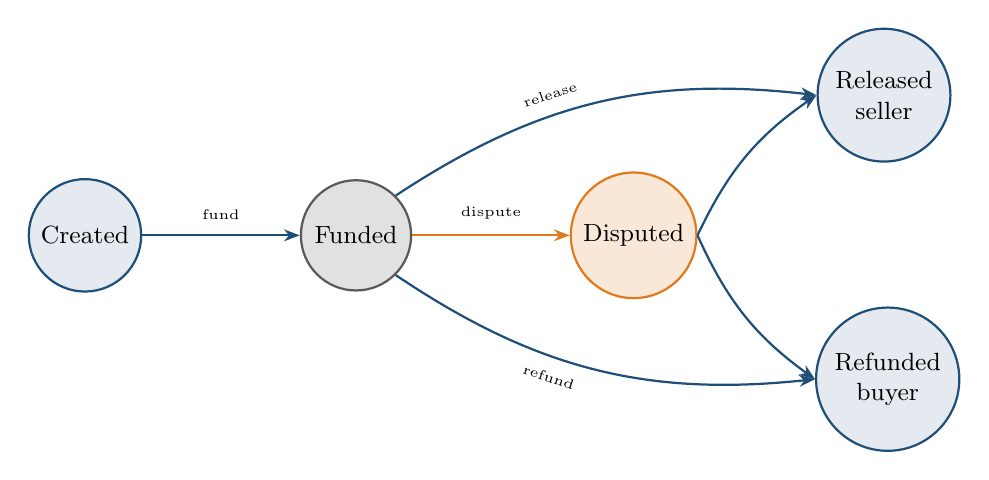
\begin{tikzpicture}[node distance=10mm and 20mm,font=\scriptsize]
  \node[node-state,node-state-normal] (c) {Created};
  \node[node-state,node-state-transition,right=of c] (f) {Funded};
  \node[node-state,node-state-alert,right=of f] (d) {Disputed};
  \node[node-state,node-state-normal,above right=6mm and 20mm of d] (rl) {Released\\seller};
  \node[node-state,node-state-normal,below right=6mm and 20mm of d] (rf) {Refunded\\buyer};
  \draw[arrow]       (c)  -- node[above=2pt,font=\tiny]{fund} (f);
  \draw[arrow-alert] (f)  -- node[above=2pt,font=\tiny]{dispute} (d);
  \draw[arrow]       (f.north east) to[bend left=20]  node[above=2pt,pos=0.4,font=\tiny,sloped]{release} (rl.west);
  \draw[arrow]       (f.south east) to[bend right=20] node[below=2pt,pos=0.4,font=\tiny,sloped]{refund}  (rf.west);
  \draw[arrow]       (d.east) to[bend left=15]  (rl.west);
  \draw[arrow]       (d.east) to[bend right=15] (rf.west);
\end{tikzpicture}}
\end{center}
{\scriptsize \textbf{业务不变式（对外承诺）}：
\begin{itemize}\setlength{\itemsep}{0pt}\setlength{\parskip}{0pt}
  \item \texttt{Created $\to$ Funded} 只能发生一次 $\to$ 用户付款不会被重复扣
  \item 终态不可逆 $\to$ 商家收到钱（Released）后平台无法撤回
  \item buyer / seller / arbiter / amount 部署后不可改 $\to$ 合约部署即承诺
\end{itemize}}
\srcnote{contracts/Escrow.sol:13--19 enum；:68--82 fund；:85--107 release/refund/dispute}
\srcnote{contracts/README.md:1--36 合约职责}
\end{frame}

\begin{frame}{合约状态 $\leftrightarrow$ 订单状态：业务对账映射}
\centering
{\small
\begin{tabular}{@{}p{22mm}p{30mm}p{50mm}@{}}
\toprule
合约状态     & 订单状态        & 触发动作 \\
\midrule
Created      & 已下单未支付    & 合约部署完成 \\
Funded       & 已支付待发货    & 买家 \texttt{fundWithOrderID} \\
（链下）     & 商家发货 / 物流 & 链下流程，不影响合约 \\
Released     & 已完成          & 买家 / 仲裁人 \texttt{release} \\
Refunded     & 已退款          & 卖家 / 仲裁人 \texttt{refund} \\
Disputed     & 售后争议        & 买家或卖家 \texttt{dispute} \\
\bottomrule
\end{tabular}}
\par\smallskip
{\small \textbf{业务约定}：链上只记"钱在谁那里"，订单详情 / 物流 / 评价 / 售后都在链下。
对账由 listener 写入 outbox 总线、与法币通道复用同一套 \texttt{order.paid} / \texttt{order.refunded} 事件型号。}
\srcnote{contracts/README.md:31--36 合约不变式}
\srcnote{service/web3/listener.go:303--311 outbox.Insert 写入 web3.payment.confirmed}
\end{frame}

\begin{frame}[fragile]{Escrow.sol 关键路径：fundWithOrderID}
\begin{lstlisting}[language=Java,firstnumber=74,
  caption={\srcnote{contracts/Escrow.sol:74--82 fundWithOrderID}}]
function fundWithOrderID(bytes32 _orderID)
    external payable onlyBuyer inState(State.Created)
{
    if (msg.value != amount) revert WrongAmount(amount, msg.value);
    orderID = _orderID;
    state = State.Funded;
    emit Funded(msg.value);
    emit PaymentConfirmed(_orderID, msg.sender, msg.value);
}
\end{lstlisting}
\small \textbf{业务对应}：
\begin{itemize}
  \item \texttt{onlyBuyer + inState(Created)}：只买家本人在"未支付"态能 fund —— 防误付 / 防重付。
  \item \texttt{msg.value != amount}：链上强校验金额，少 1 wei 也 revert —— 业务侧零信任客户端。
  \item \texttt{orderID = \_orderID}：把链下订单号写进 storage，listener 拿它 join 业务库。
  \item \texttt{emit PaymentConfirmed}：\texttt{indexed orderID} 让 listener 订一个 topic 就能精确过滤。
\end{itemize}
\end{frame}

% ============================================================
\section{业务边界与合规：gomall 在 Web3 通道里"不做什么"}
% ============================================================

\begin{frame}{业务边界（显式声明）：Web3 通道里 gomall 不做的事}
诚实列出，对外承诺：
\begin{itemize}
  \item \textbf{不真上链}：合约源码 + Go binding 完整，MVP 阶段默认 \texttt{WEB3\_RPC\_URL} 不设，listener 不启动；订单仍可签名挂 pending（路线图阶段切真链）。
  \item \textbf{不托管钱包}：用户私钥永远在用户自己的钱包，平台没有"代用户签名"能力。
  \item \textbf{不做币种兑换}：用户拿 ETH 付款，商家收 ETH；想换 USDC 用户自己换。
  \item \textbf{不做跨链桥}：每条链独立部署 escrow，不接 CCIP / LayerZero / Wormhole（行业过去 3 年桥被盗 \$25B+，风险太大）。
  \item \textbf{不发 NFT 票据}：订单凭证仍是链下 DB 行，不上链 NFT。
  \item \textbf{不发自有 stablecoin}：用市场上已有的（USDC / USDT / DAI）。
  \item \textbf{不做 KYC / AML 自家方案}：制裁名单过滤路线图阶段接 Chainalysis / TRM Labs API。
\end{itemize}
\srcnote{README.md:69--80 业务边界对应章节}
\srcnote{service/web3/listener.go:113--117 envRPCURL 未设静默不启动}
\end{frame}

\begin{frame}{合规边界：链上身份 vs 实名监管}
\textbf{Web3 合规是 gomall MVP 阶段刻意延后的话题}，但路线图必须想清楚：
\begin{itemize}
  \item \textbf{钱包地址 $\neq$ 实名}：链上地址默认匿名，监管要求（FATF Travel Rule）\$3{,}000+ 交易必须 KYC。
  \item \textbf{阶梯式 KYC 路线图}：\$100 以下免；\$100--\$3{,}000 邮箱 + 电话；\$3{,}000+ 强制身份证 + 人脸。
  \item \textbf{OFAC / 制裁名单}：Tornado Cash 等地址必须拒绝；落地 = 接 Chainalysis / TRM Labs API，验签后写 outbox 前过滤。
  \item \textbf{多签仲裁是合规可审计的关键}：单签 arbiter 无法对监管解释"为什么这笔 release"；2-of-3 多签 + 合规岗签名可留下链上证据。
\end{itemize}
\vspace{1mm}
\small \textbf{业务声明}：gomall MVP 阶段单笔 \$100 以内、单 EOA arbiter；超过 \$100 或托管总额超 \$10k
强制切 Gnosis Safe 2-of-3 多签，不重新部署 Escrow，只在新订单的 constructor 里换 arbiter 地址。
\srcnote{internal/payment/service\_crypto.go:116--124 验签后 / 写 outbox 前，是合规过滤的天然插入点}
\srcnote{contracts/Escrow.sol:10 arbiter immutable；contracts/README.md:101--102 多签建议}
\end{frame}

\begin{frame}{业务承诺（SLO）：Web3 通道的对外承诺}
\begin{tabular}{@{}lll@{}}
\toprule
环节 & SLO 目标 & 当前实测 \\
\midrule
nonce 颁发 & p99 < 100ms & Redis SET + 5min TTL \\
验签 + outbox 写入 & p99 < 200ms & DB 事务 + Redis SETNX \\
链上事件 $\to$ outbox 写入 & 5min 内 & catch-up + dedupe \\
listener 重启 catch-up & 5min 内 & FilterLogs 批量回放 \\
RPC 全断时主流程可用 & 100\% & 法币通道独立，Web3 静默降级 \\
\bottomrule
\end{tabular}
\vspace{2mm}
\small \textbf{压测对照}（参 \texttt{stressTest/REPORT.md}）：法币 \texttt{/paydown} 走幂等中间件，
跑出 \textbf{50K RPS / p95 2.33ms}（50VU × 15s 同 Idempotency-Key 累计 755{,}033 次请求 $\to$ DB 1 笔订单）。
Web3 \texttt{/paydown/crypto} 复用同一套幂等 + 事务 + outbox 体系，业务路径开销 < 5ms（不含链上等待）。\\
\textbf{业务保证的根基}：链是不可靠通道但 outbox 总线可靠。listener 写入 outbox 后，对账 / 通知 / 状态推进
全部走与法币通道相同的 \texttt{web3.payment.confirmed} $\to$ \texttt{order.paid} 链路（deck 11 同款）。
\srcnote{stressTest/REPORT.md:34--87 /orders/create 与 /paydown 路径的 RPS / p95 / max 数据}
\srcnote{README.md:54--65 P0 核心交易 SLO 99.95\% / p99 < 500ms}
\end{frame}

% ============================================================
\section{各角色视角 + 路线图}
% ============================================================

\begin{frame}{各角色视角：业务侧关心的全图}
\begin{tabular}{@{}lll@{}}
\toprule
角色   & 关心               & 看哪里 \\
\midrule
用户   & 钱安全吗            & 合约不变式 + 不托管承诺 + 退款流程 \\
商家   & 何时到账            & 链上确认数 + release 时机 + gas 自付 \\
客服   & 链上失败咋办        & W3-* 业务码对应处理 SOP \\
运营   & 开通道转化率多少    & 新用户群（DeFi / 跨境 / 大额）数据 \\
SRE    & 链断了主流程挂吗    & 静默降级 + listener 重连 + outbox 兜底 \\
法务   & 合规边界            & 路线图阶段：KYC + 多签 + 司法管辖 \\
财务   & 链上链下对账        & outbox 统一总线 + channel 标识 \\
\bottomrule
\end{tabular}
\vspace{2mm}
\small \texttt{outbox} 总线让财务对账拿到\textbf{统一格式}事件：channel = fiat / web3-eth / web3-usdc，
按 \texttt{order\_id} join。\textbf{业务边界}：链 / 币 / gas 三选一组合，
MVP 推荐 \textbf{L2 + ETH 原生币 + 用户自付 gas}，正式运营后逐步上稳定币 + gas 补贴 + 多链路由。
\srcnote{service/web3/listener.go:303--311 outbox.Insert 与法币通道复用同一总线}
\srcnote{README.md:21--29 5 角色 + 业务全景表}
\end{frame}

\begin{frame}{Arbiter 多签升级路线图}
\begin{tabular}{@{}lll@{}}
\toprule
阶段 & arbiter 形态  & 适用金额上限 \\
\midrule
MVP  & 平台 EOA     & 等值 \$100 以内 \\
2    & 2-of-3 多签  & 等值 \$10{,}000 以内（Gnosis Safe） \\
3    & DAO 治理     & 超大额 / 跨组织 \\
\bottomrule
\end{tabular}
\vspace{2mm}
\textbf{业务驱动}：
\begin{itemize}
  \item MVP 单 EOA 私钥放运营手里，丢私钥 / 私钥被盗 = 所有 Disputed 订单卡死 + 平台跑路风险。
  \item 单笔 \$10{,}000+ 用户不会接受"平台单签拍板"；监管也不接受。
  \item 升级关键：\textbf{切换不需要重新部署 Escrow}，只在新订单的 constructor 里传 Safe 地址即可（旧订单 arbiter immutable 保持不变）。
  \item Safe 是合约钱包，对外暴露 \texttt{execTransaction}，N-of-M 签名后转发 calldata；从 Escrow 看 \texttt{msg.sender} 就是 Safe 地址。
\end{itemize}
\srcnote{contracts/Escrow.sol:10 arbiter immutable；:57--65 constructor}
\srcnote{contracts/README.md:101--102 arbiter 推荐多签}
\end{frame}

\begin{frame}{从技术决策回看业务依据}
\small
\begin{tabular}{@{}ll@{}}
\toprule
技术选择                        & 业务依据 \\
\midrule
EIP-191 personal\_sign          & 钱包弹窗让用户看到明文，钓鱼可识别 \\
nonce 走 Redis Lua 原子         & 一次性消费，防同链重放 \\
chainID 入签名消息              & 防 mainnet / L2 跨链重放 \\
合约 emit PaymentConfirmed       & listener 订一个 event 就能精确对账 \\
listener 写 outbox 而非直推订单 & 与法币通道复用一套对账 \\
SETNX 72h 事件级幂等            & reorg / 重连 / 重启业务侧无感 \\
arbiter 走多签路线              & 单签平台跑路风险对外无法解释 \\
\texttt{WEB3\_RPC\_URL} 未设静默降级 & 链不通时主流程仍可用 \\
\bottomrule
\end{tabular}
\vspace{1mm}
\keypoint{Web3 的业务价值不在"潮"，在于\textbf{把"第三方信任"从"中介机构"换成"可审计代码"} —— 这对加密原生 / 跨境 / 大额三类订单都是真痛点。}
\srcnote{routes/router.go:122--136 Web3 路由接入位}
\srcnote{service/web3/listener.go:113--117 静默降级入口}
\end{frame}

% ============================================================
\appendix
% ============================================================

\begin{frame}{面试 Q\&A（上）}
\textbf{Q1}：链 reorg 把已 release 的资金撤销了怎么办？\\
\hspace{4mm}\small A：风控阈值（确认数）由商家自己设；mainnet 大额走 32 块 = 1 epoch finalize；
L2 大额等回 L1 finalize。listener 监听 \texttt{lg.Removed} 跳过 reorg log，订单状态不会被错误推进；
若商家已基于浅确认提前发货，arbiter 介入 + 商家走链下追款，平台不兜底。\\
\srcnote{service/web3/listener.go:218--221}

\vspace{1.5mm}
\textbf{Q2}：用户钱包私钥丢了订单怎么处理？\\
\hspace{4mm}\small A：链上没有"重置密码"。资金在 Funded 态可由仲裁人核实身份后 refund 到新地址；
已 Released 给商家则只能走链下补偿。这就是为什么 MVP 阶段单笔 \$100 以内的业务限制 —— 把单笔损失上限封住。\\
\srcnote{contracts/Escrow.sol:94--100 refund 入口可由 arbiter 触发}

\vspace{1.5mm}
\textbf{Q3}：法币和 Web3 两套通道怎么共存？\\
\hspace{4mm}\small A：路由层并行挂载 \texttt{/paydown}（法币）和 \texttt{/paydown/crypto}（Web3），
事件层都写入同一条 outbox 总线（事件加 channel 字段：fiat / web3-eth / web3-usdc），
对账任务按 \texttt{order\_id} join 法币入账 + 链上 confirmed event。下游消费者完全不感知通道差异。\\
\srcnote{routes/router.go:122--136 两条路由并行}

\vspace{1.5mm}
\textbf{Q4}：MVP 阶段为什么默认不真连链？\\
\hspace{4mm}\small A：(1) RPC 节点 + gas 是真金白银，跑通业务流程不需要烧；(2) 真上链需要第三方合约审计 + 切多签 + 接 KYC，是路线图里独立 PR；
(3) 静默降级保证合约 + binding + listener 全部代码在路径上跑过单测，env 一开就上链。\\
\srcnote{service/web3/listener.go:113--117 envRPCURL 未配置静默不启动}
\srcnote{README.md:75--80 业务边界显式列出"不真上链"}
\end{frame}

\begin{frame}{面试 Q\&A（中）}
\textbf{Q5}：客服遇到"用户付款半小时还没到"咋办？\\
\hspace{4mm}\small A：分四步问 ——
(1) 是哪条链（mainnet 拥堵 1--2 小时正常，L2 超 5 分钟才算异常）；
(2) 钱包侧 tx 是否真的广播了（用户给 txhash）；
(3) SRE 后台 grep outbox 是否有 \texttt{web3.payment.pending}（=后端验签通过）；
(4) listener 日志该 txhash 是否被消费。三段都能查 = 90\% 事故可定位。\\
\srcnote{repository/cache/web3.go:21--26 Web3PendingTTL=30min}
\srcnote{internal/payment/service\_crypto.go:151--154 SetWeb3Pending}

\vspace{1.5mm}
\textbf{Q6}：为什么 nonce 必须后端发，前端自己生成不行？\\
\hspace{4mm}\small A：前端可生成的 nonce 后端没法保证唯一性也没法做时效控制；攻击者拿到一次有效签名后可无限重放。
后端 Redis + Lua 原子 GET+DEL 才能保证"一次性"。\\
\srcnote{repository/cache/web3.go:60--89 consumeNonceScript}

\vspace{1.5mm}
\textbf{Q7}：listener 进程重启会不会丢事件？业务侧怎么对外解释？\\
\hspace{4mm}\small A：不会。\texttt{loadLastBlock} 从 Redis 拿最后处理块号，\texttt{catchUp(last+1, head)} 批量回放停机期事件，
再叠加 SETNX 72h 幂等，重启不会重做也不会丢。\textbf{对外承诺}："Web3 通道掉单率为 0，最坏情况是延迟 5 分钟到账"。\\
\srcnote{service/web3/listener.go:232--248 catchUp；:316--326 tryClaim}

\vspace{1.5mm}
\textbf{Q8}：Web3 通道为什么需要 gomall 的幂等中间件 + outbox？\\
\hspace{4mm}\small A：钱包用户在确认 tx 时常因 gas 不够重试 $\to$ 后端 \texttt{/paydown/crypto} 收到两次同 Idempotency-Key 请求 $\to$ 幂等中间件让第二次直接 replay 第一次结果。
事务 + outbox 保证"验签通过"与"事件落地"同生共死，下游不会收到孤儿事件。\\
\srcnote{routes/router.go:132--136 paydown/crypto 套幂等中间件}
\srcnote{internal/payment/service\_crypto.go:129--148 事务内写 outbox}
\end{frame}

\begin{frame}{面试 Q\&A（下）}
\textbf{Q9}：单签 arbiter 多久应该切多签？\\
\hspace{4mm}\small A：单笔 \$100 以内可继续单 EOA；超过 \$100 或托管总额超 \$10k 强烈建议切 2-of-3 Gnosis Safe；
切换不需重新部署 Escrow（旧订单 arbiter immutable 保持），新订单 constructor 里传 Safe 地址即可。
监管视角也只接受多签 —— 单签平台无法对外解释"为什么这笔 release"。\\
\srcnote{contracts/Escrow.sol:57--65 constructor；contracts/README.md:101--102}

\vspace{1.5mm}
\textbf{Q10}：合规（OFAC）名单上的钱包地址来 paydown 怎么拦？\\
\hspace{4mm}\small A：在 \texttt{VerifyAndPark} 第 2 段（验签后、写 outbox 前）插一个 Chainalysis / TRM Labs 黑名单查询，
命中返回 \texttt{W3-COMPLIANCE-REJECTED} + 客服话术；不修改合约，纯链下卡口，合规可独立审计。
路线图阶段，MVP 不接（业务边界声明）。\\
\srcnote{internal/payment/service\_crypto.go:116--124 验签后是天然过滤点}

\vspace{1.5mm}
\textbf{Q11}：RPC 节点全断 30 分钟，业务怎么办？\\
\hspace{4mm}\small A：listener 进入退避重连（1s $\to$ 60s 封顶），期间链上事件不消费；新增订单仍可签名挂 pending（验签不依赖 RPC）；
法币通道完全不受影响。30 分钟后 RPC 恢复，\texttt{catchUp(last+1, head)} 自动补齐所有漏掉的事件，
business 侧最终一致性 SLO 守住 5 分钟（漏的 30 分钟事件在重连后 5 分钟内全部 outbox 化）。\\
\srcnote{service/web3/listener.go:155--175 run() 退避；:232--248 catchUp}

\vspace{1.5mm}
\textbf{Q12}：Web3 通道对 gomall 业务最大的价值是什么？一句话总结。\\
\hspace{4mm}\small A：补齐法币吃不下的三类订单 —— 加密原生用户（钱包里无卡）、跨境（避 1--3\% 手续费 + T+1）、
大额托管（信任锚从银行换成可审计代码）。\textbf{不是替代法币，是拓客}。
通道开了就有，不开就少这三类用户。\\
\srcnote{README.md:69--80 业务边界}
\srcnote{routes/router.go:122--136 两条通道并行}
\end{frame}

\begin{frame}{代码位置一览（上）}
\small
\begin{description}
  \item[Escrow 合约 + 状态机]\srcnote{contracts/Escrow.sol:7--113}
  \item[immutable 参数 / custom error]\srcnote{contracts/Escrow.sol:8--11；:32--35}
  \item[fundWithOrderID 入金]\srcnote{contracts/Escrow.sol:76--82}
  \item[release / refund / dispute]\srcnote{contracts/Escrow.sol:85--107}
  \item[钱包验签 EIP-191]\srcnote{pkg/web3/signature/verify.go:31--82}
  \item[Nonce 颁发 + 验签业务]\srcnote{internal/payment/service\_crypto.go:49--160}
  \item[签名消息模板 / chainID 防重放]\srcnote{internal/payment/service\_crypto.go:39--46}
  \item[Web3 Redis 协议（nonce/pending）]\srcnote{repository/cache/web3.go:21--101}
  \item[Lua 原子 GET+DEL]\srcnote{repository/cache/web3.go:60--89}
\end{description}
\end{frame}

\begin{frame}{代码位置一览（下）}
\small
\begin{description}
  \item[链上 listener 主循环]\srcnote{service/web3/listener.go:108--230}
  \item[catch-up 补块]\srcnote{service/web3/listener.go:232--248}
  \item[reorg 跳过]\srcnote{service/web3/listener.go:218--221}
  \item[事件级幂等 SETNX 72h]\srcnote{service/web3/listener.go:296--326}
  \item[last\_block 持久化]\srcnote{service/web3/listener.go:328--352}
  \item[退避重连]\srcnote{service/web3/listener.go:360--377 backoff 1s$\to$60s}
  \item[静默降级（env 未设跳过）]\srcnote{service/web3/listener.go:113--117}
  \item[Outbox 总线写入]\srcnote{internal/payment/service\_crypto.go:129--144}
  \item[API 路由接入位]\srcnote{routes/router.go:122--136}
  \item[crypto handler]\srcnote{internal/payment/handler\_crypto.go:14--52}
  \item[合约部署 / 多签建议]\srcnote{contracts/README.md:1--104}
\end{description}
\keypoint{现状：合约 + binding 在 feat/web3-escrow PR；\textbf{MVP 默认未上链}（\texttt{WEB3\_RPC\_URL} 不设），上线前需第三方审计 + 切多签 + 接 KYC。}
\end{frame}

\end{document}
